\documentclass[oneside,a4paper,11pt,explicit]{book}
\usepackage[utf8]{inputenc}
\usepackage{icecream}
\usepackage[english]{babel}
\addto\captionsenglish{\renewcommand{\chaptername}{}}
\usepackage[accsupp]{axessibility}  % improves PDF readability for those with disabilities.
\usepackage[colorlinks = true,urlcolor  = blue,linkcolor = blue]{hyperref}
\usepackage{setspace}
\usepackage{listings}
\usepackage[most]{tcolorbox}
\usepackage{minitoc}
\usepackage{multicol}


\renewcommand{\mtifont}{\large\sffamily}
\renewcommand{\mtcfont}{\small\sffamily}
\renewcommand{\mtcSfont}{\small\sffamily}
\renewcommand{\mtcSSfont}{\small\sffamily}
\renewcommand{\mtcSSSfont}{\small\sffamily}
\mtcsetpagenumbers{minitoc}{off} % turn off page numbering in minitocs
\addto{\captionsenglish}{% Making babel aware of special titles
	\renewcommand{\mtctitle}{Quick Links To Sections}
}
\setlength{\fboxrule}{5pt}
\setlength{\fboxsep}{4pt}

\definecolor{IceCreamLeaf}{rgb}{0.4, 0.639215686274, 0.4}
\definecolor{IceCreamOrbit}{rgb}{0.803921568627451, 0.3607843137254902, 0.3607843137254902}

\title{I.C.E.C.R.E.A.M. Tutorials}
\subtitle{\small Observing Earth from Above (Env 329) v24.06 \\
	\small Schmid College of Science and Technology, Chapman University}
\date{\today}

%% DOCUMENT
\setstretch{1.25}
\makeatletter
\begin{document}

\dominitoc

%\tableofcontents

\setcounter{chapter}{9} %Insert (Tutorial Number-1) Here; example for tutorial 4, enter 3

\chapter{Estimating Coupled Carbon and Water Cycling in Plants} %Enter Tutorial Name Here

\vspace{-2em}

\minitoc

\hrule

\vspace{1em}

\begin{tcolorbox}[enhanced,frame style image=blueshade.png,
	opacityback=0.75,opacitybacktitle=0.25,
	colback=blue!5!white,colframe=blue!75!black,title={\Large \textbf{Objectives:}}]
	\large
	\begin{enumerate}
		\item Identify how the different components of evapotranspiration that ECOSTRESS reports can be used to describe ecosystem function.
		\item Develop hypotheses to compare two ecosystems in the context of natural climate solutions and create a NASA worthy map to address your hypotheses.
	\end{enumerate}
\end{tcolorbox}

\clearpage

%%%%%%%%%%%%%%%%%%%%%%%%%%%%%%%%%% Change Header to Have a Smaller Logo for Remainder of the Document
\fancyhead{}
\fancyhead[C]{\begin{tikzpicture}[overlay, remember picture]
		\fill[Blue2] (current page.north west) rectangle ($(current page.north east)+(0,-1in)$);
		\node[anchor=north west, text=white, font=\Large, minimum size=1in, inner xsep=5mm, align=left] at (current page.north west) {\bf{\MakeUppercase{\@title}}\\\@subtitle};
		\node[anchor=north east, minimum size=1in, inner xsep=5mm] at (current page.north east) {\includegraphics[scale=.125]{ICECREAM_Logo.png}};\end{tikzpicture}}
%%%%%%%%%%%%%%%%%%%%%%%%%%%%%%%%%%

\noindent\fbox{\begin{minipage}{.9665\textwidth}
			
	\vspace{1em}
	\begin{center}
		\textbf{\Large \underline{Motivation For Today's Tutorial : Natural Climate Solutions}}
	\end{center}
	
	\addcontentsline{toc}{section}{Motivation : Natural Climate Solutions}

	\vspace{1 em}
	
	\centerline{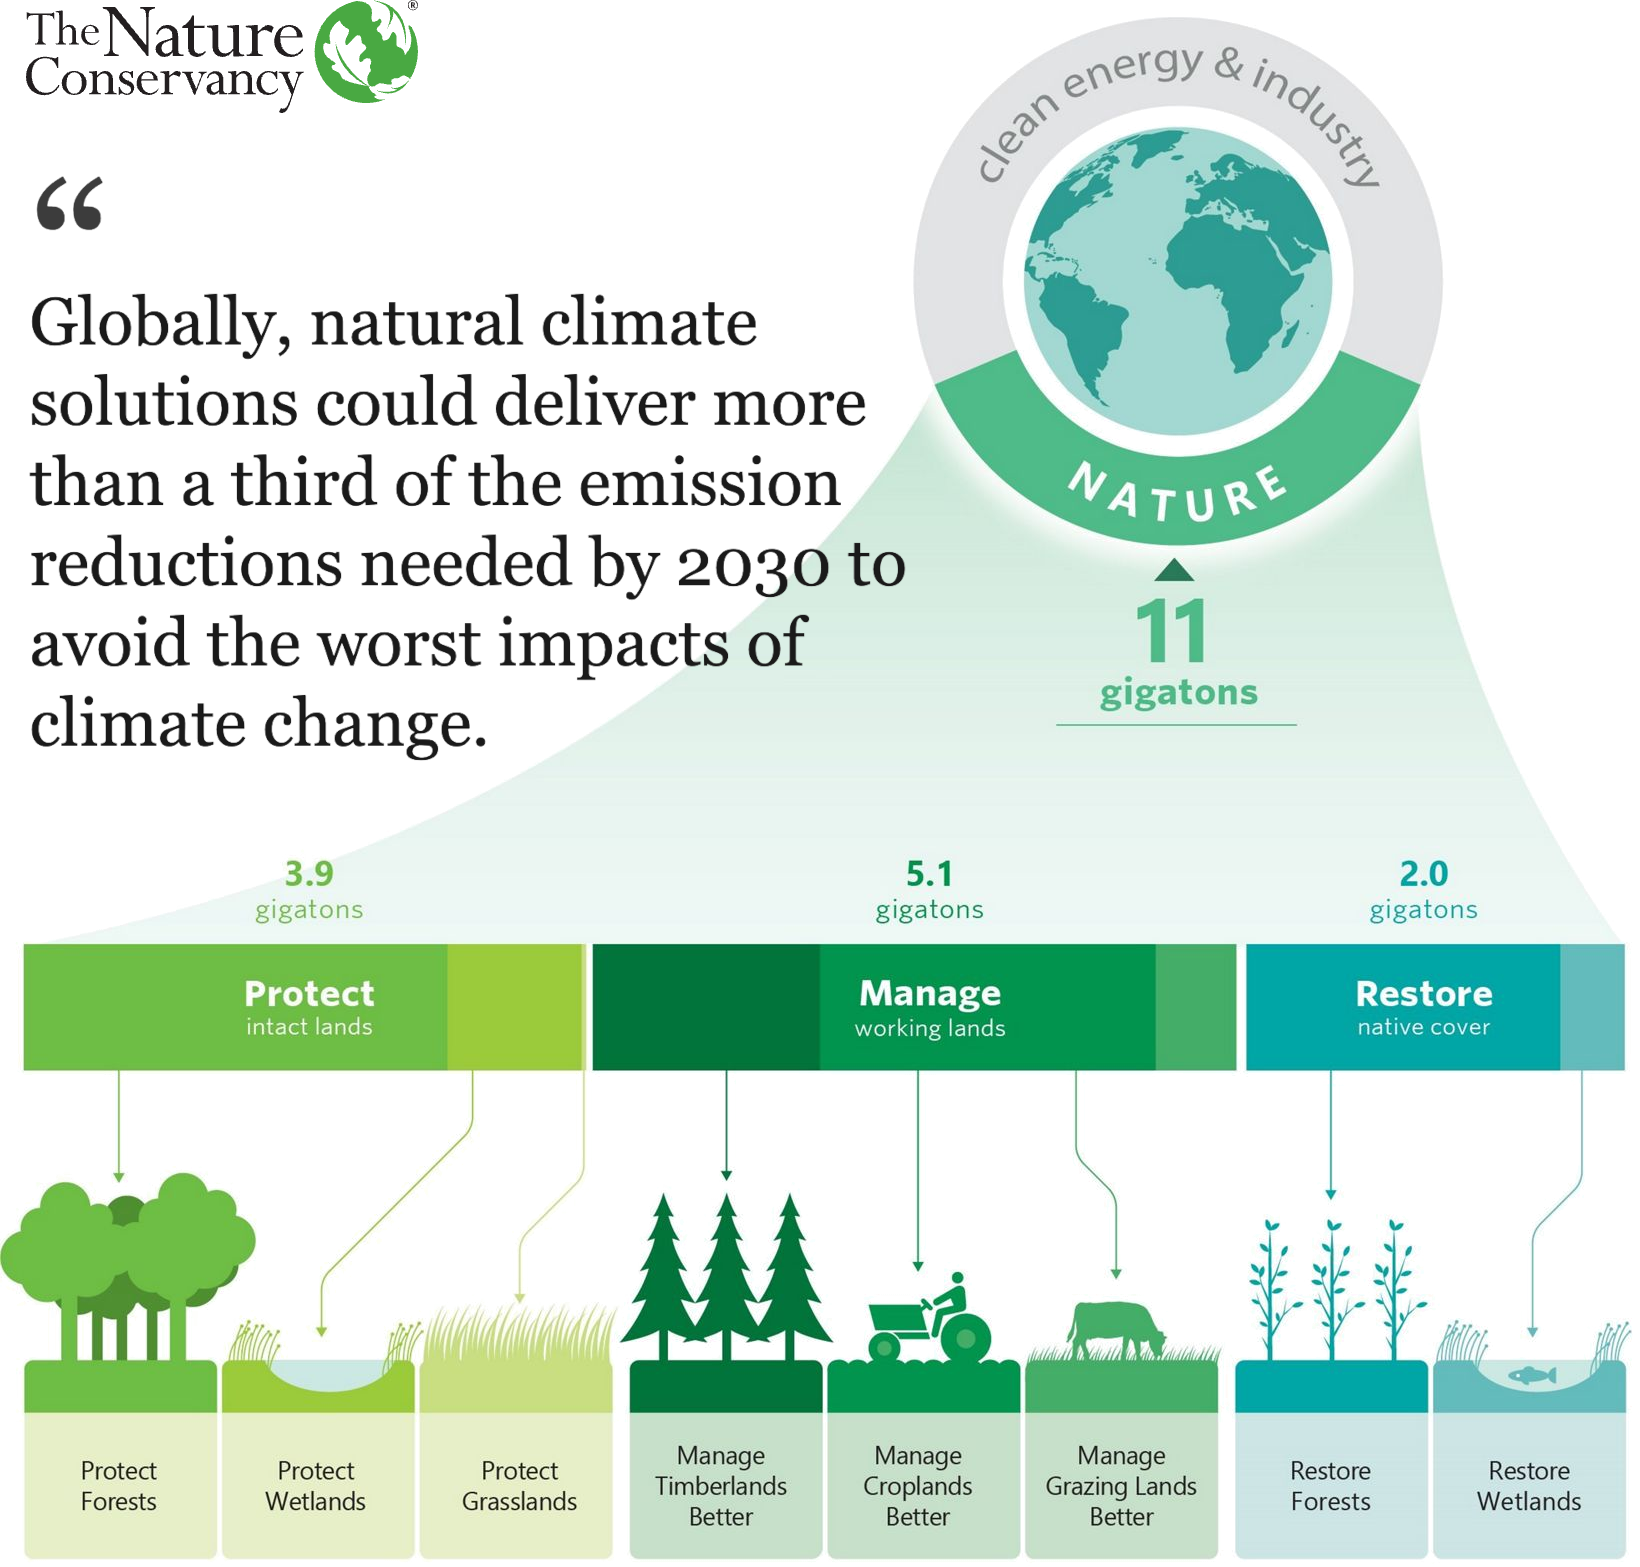
\includegraphics[width=.975\textwidth]{NCS.png}}
	
	\vspace{1 em}
	
Natural climate solutions are actions that scientists have identified to protect, manage, and restore nature to reduce greenhouse gas emissions and store carbon. Combined with the transition away from fossil fuels, natural climate solutions offer immediate and cost-effective ways to address the climate crisis, while also supporting healthy and thriving ecological communities and ecosystems. 
	
	\vspace{.5 em}

	Examples of natural climate solutions include reforestation, agriculture and timber management, and protection of ecosystems known to capture and store large amounts of carbon. Less carbon in the atmosphere reduces the greenhouse effect, which is needed to achieve the goal of the Paris Climate Agreement of maintaining warming below 2 $^\circ$ C. Climate scientists use remote sensing data, such as evapotranspiration and water use efficiency from ECOSTRESS, to help assess the impact of natural climate solution actions.

	\vspace{.5em}

\end{minipage}}

\section{Accessing ECOSTRESS ET Component \& WUE Data through A$\rho\rho$EEARS}

\subsection{ECOSTRESS Evapotranspiration (ET) \& Water Use Efficiency (WUE) Data Variables}

\vspace{.5em}

\centerline{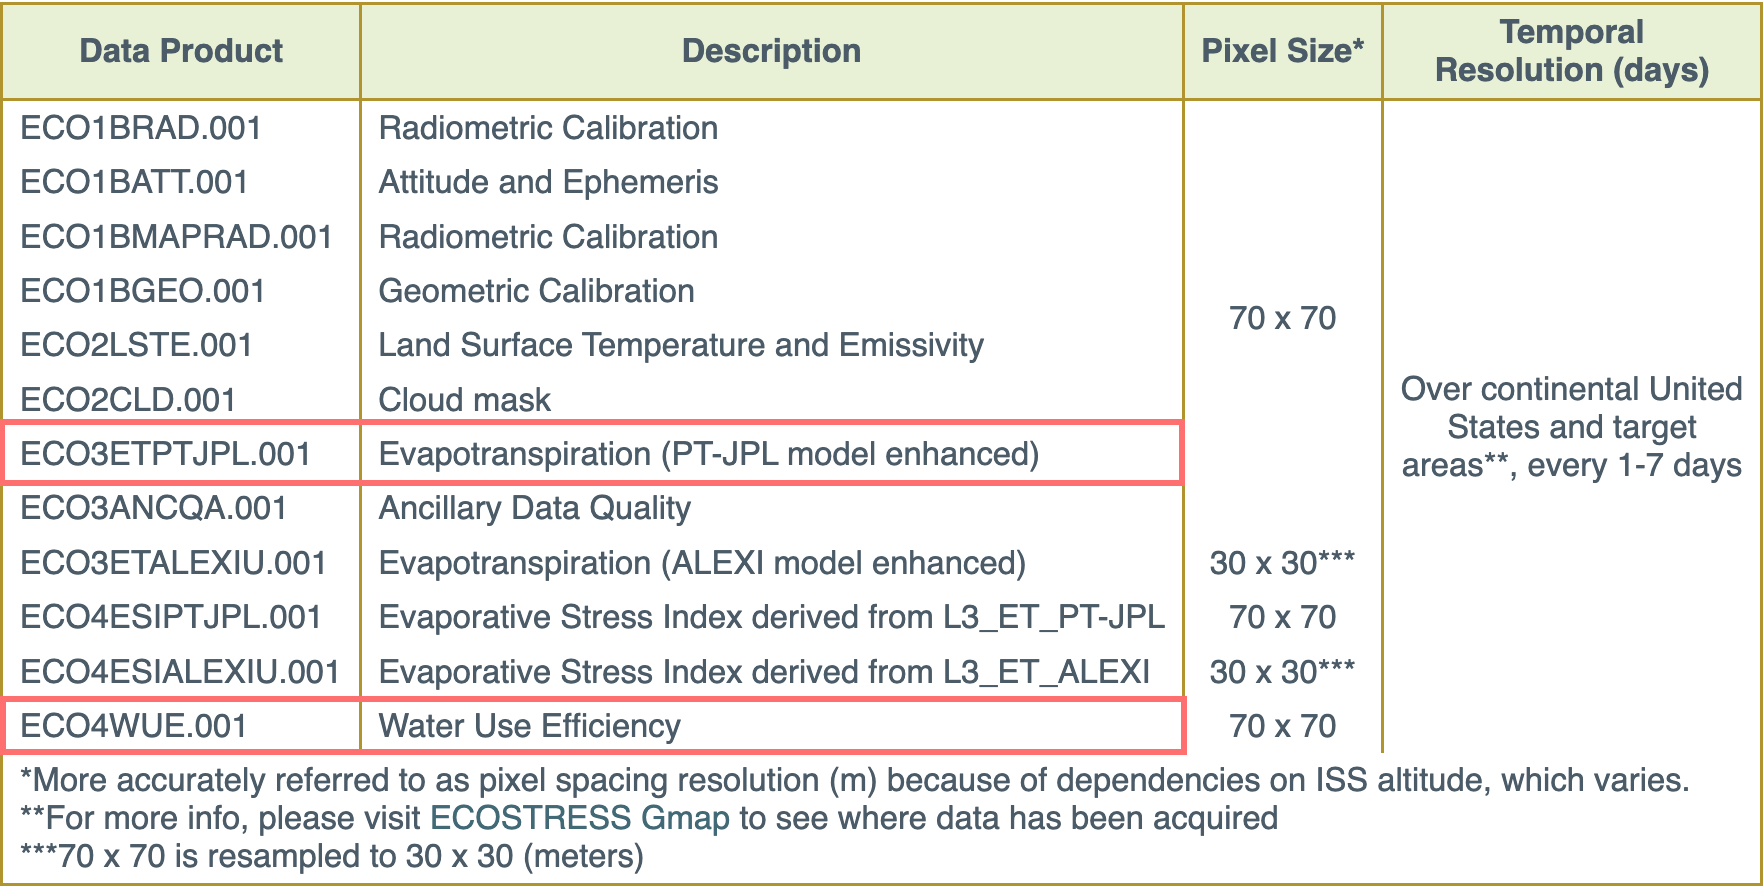
\includegraphics[width=.75\textwidth]{ECOSTRESS_DataProducts.png}}

\vspace{.5em}

In the last tutorial, we learned that ECOSTRESS uses land surface temperatures to estimate evapotranspiration (ET), the sum of all processes that return water from the land surface to the atmosphere (evaporation + transpiration). The Level 3 (ECO3) ET data that we worked with last time ($ET_{inst}$ \& $ET_{daily}$) represent the total ET, but ECOSTRESS also has data that allow us to track the individual components of ET:

\vspace{.5em}

\centerline{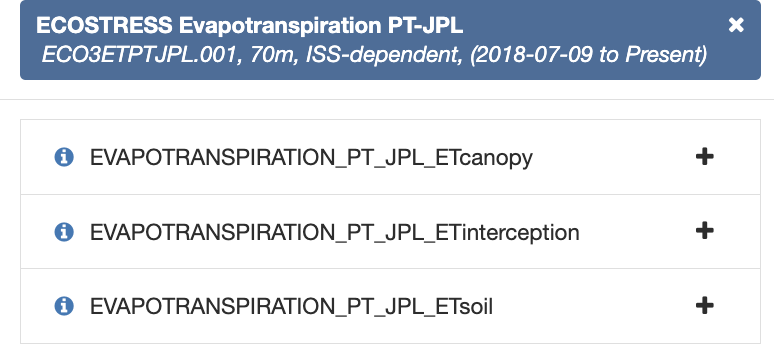
\includegraphics[width=.6\textwidth]{ETjplComponents.png}}

\begin{itemize}
	\item $ET_{canopy}$ = transpiration of water from the leaves (through stomata in higher plants)
	\item $ET_{interception}$ = evaporation of water off of the surface of the plants
	\item $ET_{soil}$ = evaporation of water from the soil
\end{itemize}

Water use efficiency (WUE), or the amount of carbon plants take up per unit of water lost, is a Level 4 (ECO4) ECOSTRESS data product:

\vspace{.5em}

\centerline{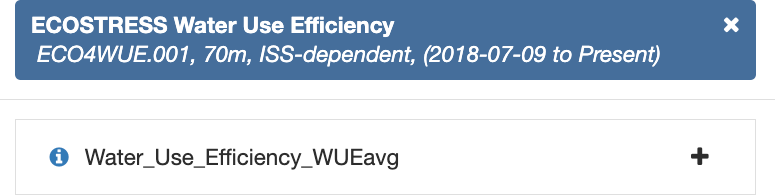
\includegraphics[width=.6\textwidth]{WUEecostress.png}}

\addcontentsline{toc}{subsection}{Today's Study Location : Southern Pine Forests}

\begin{tcolorbox}[colback=yellow!5!white,colframe=IceCreamLeaf,title=\textbf{Southern Pine Forests}]
	\begin{multicols}{2}

	\centerline{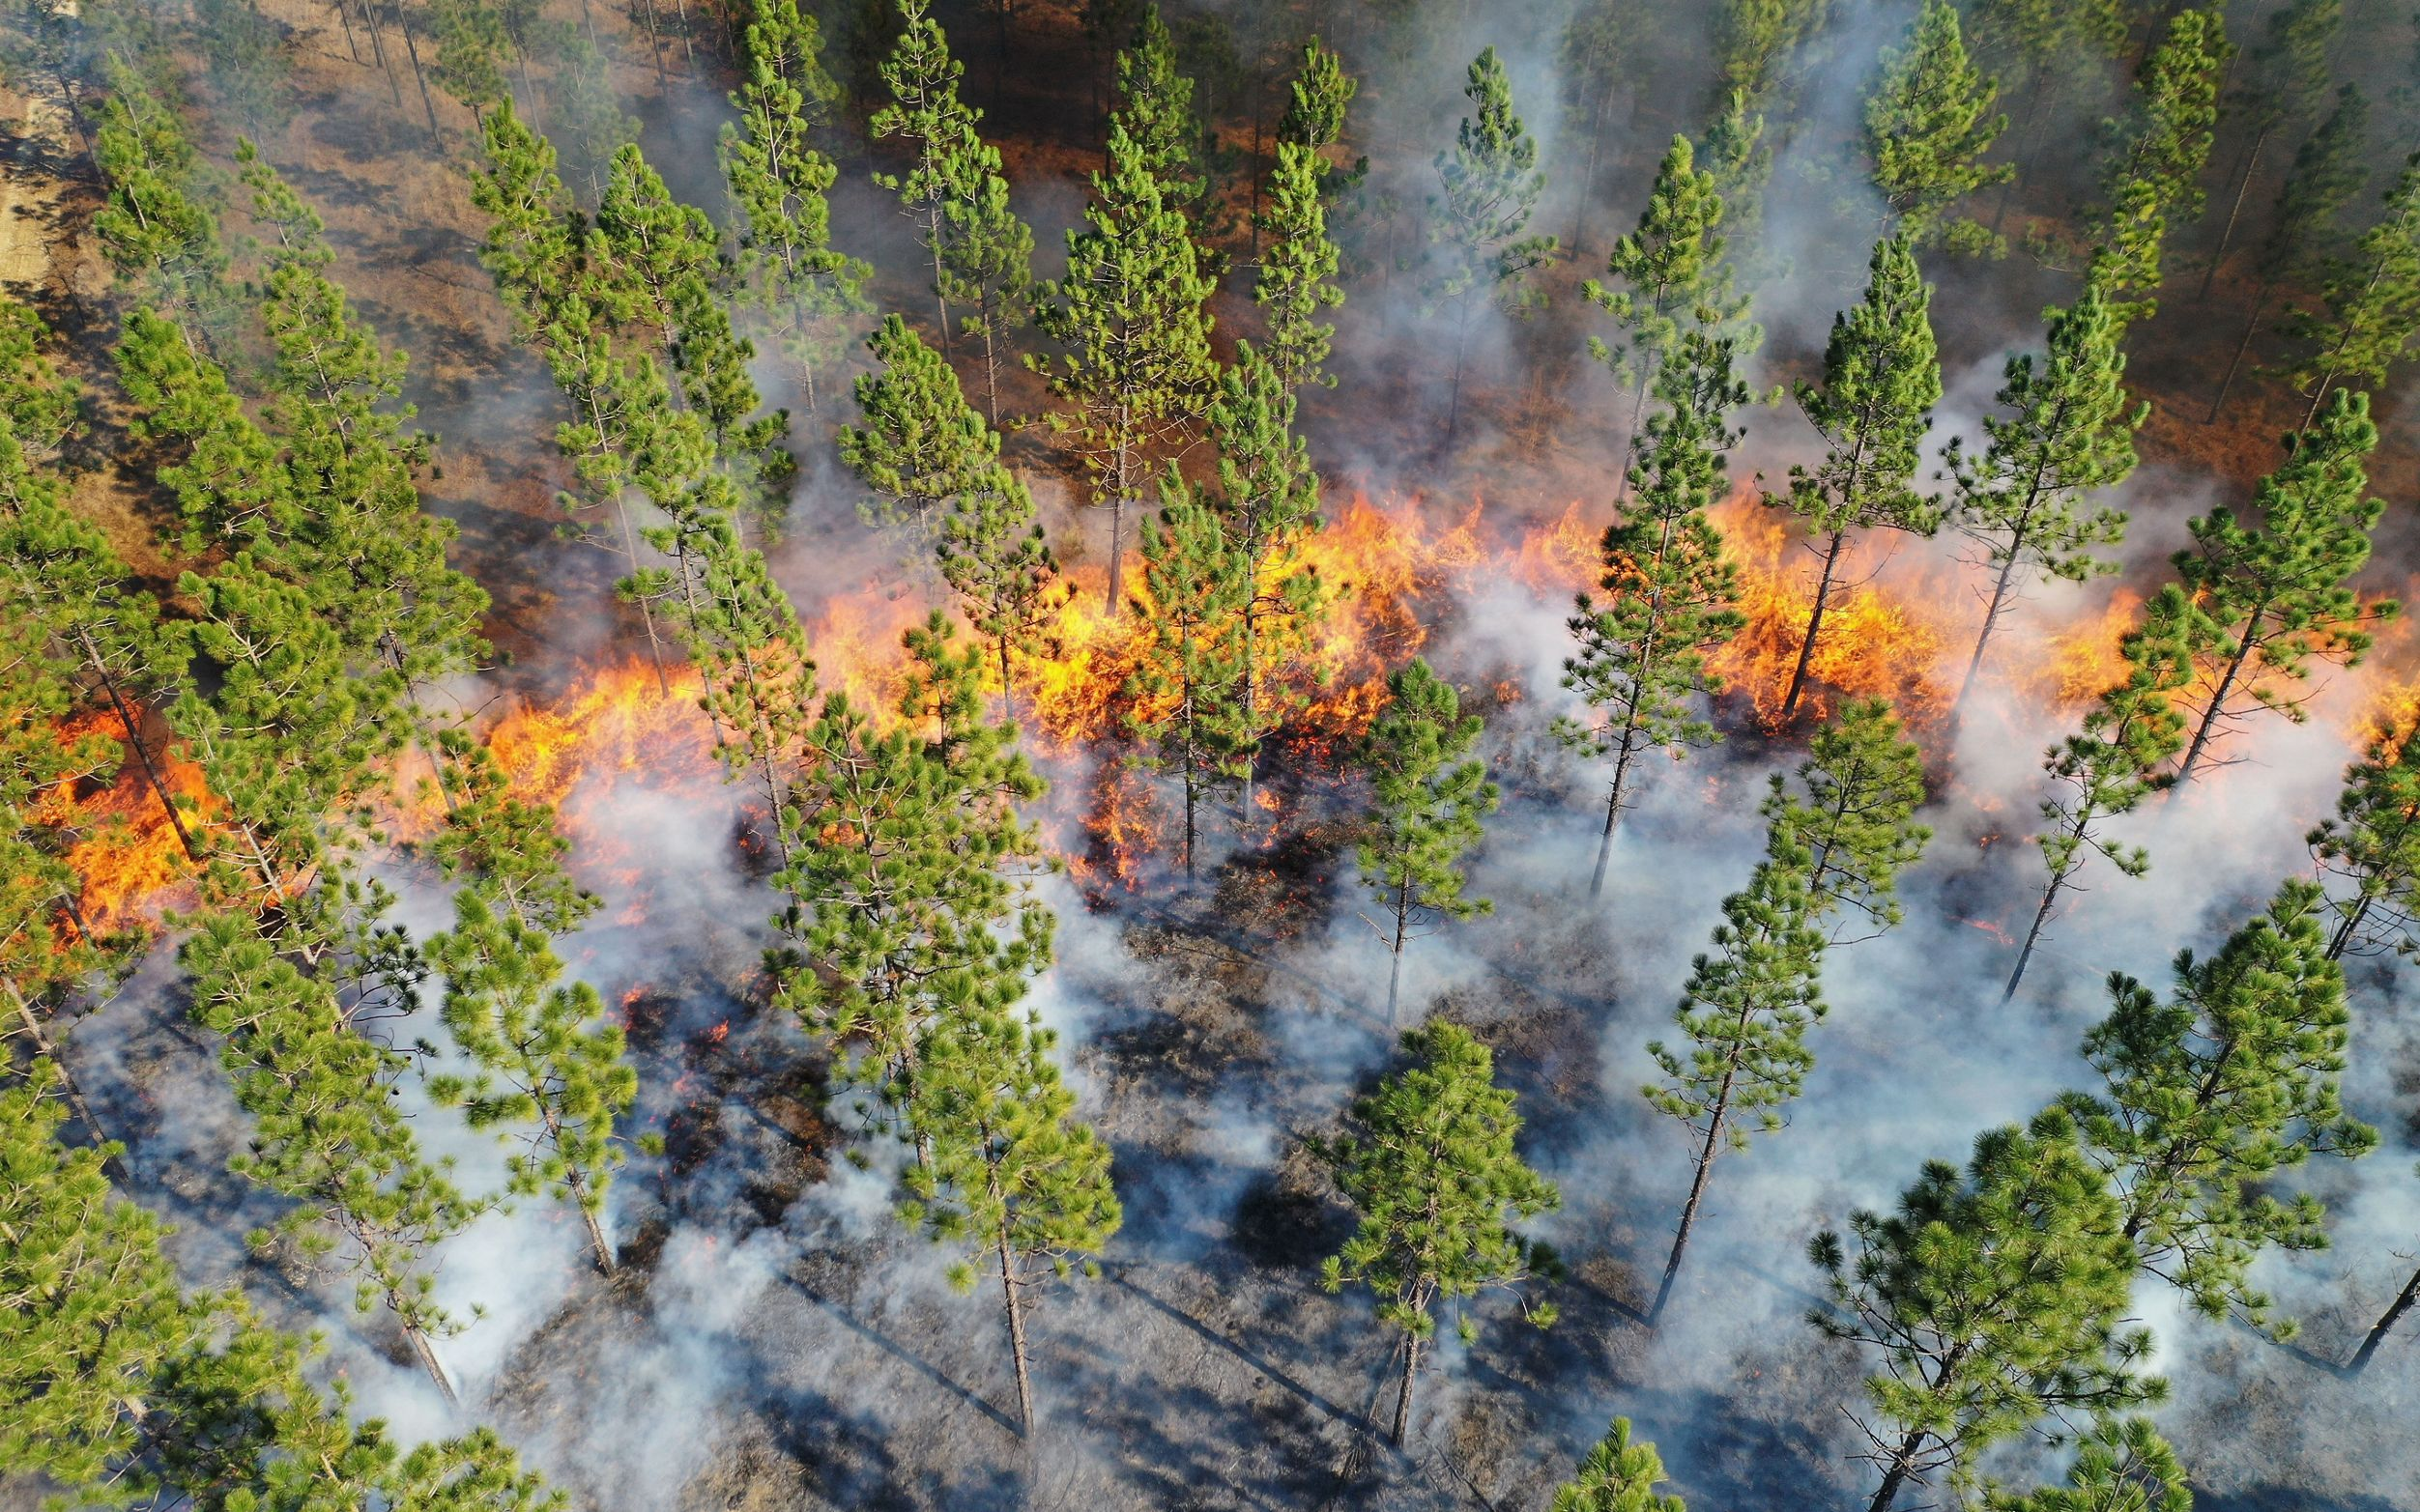
\includegraphics[width=.975\columnwidth]{SPineBurn.jpeg}}
	\centerline{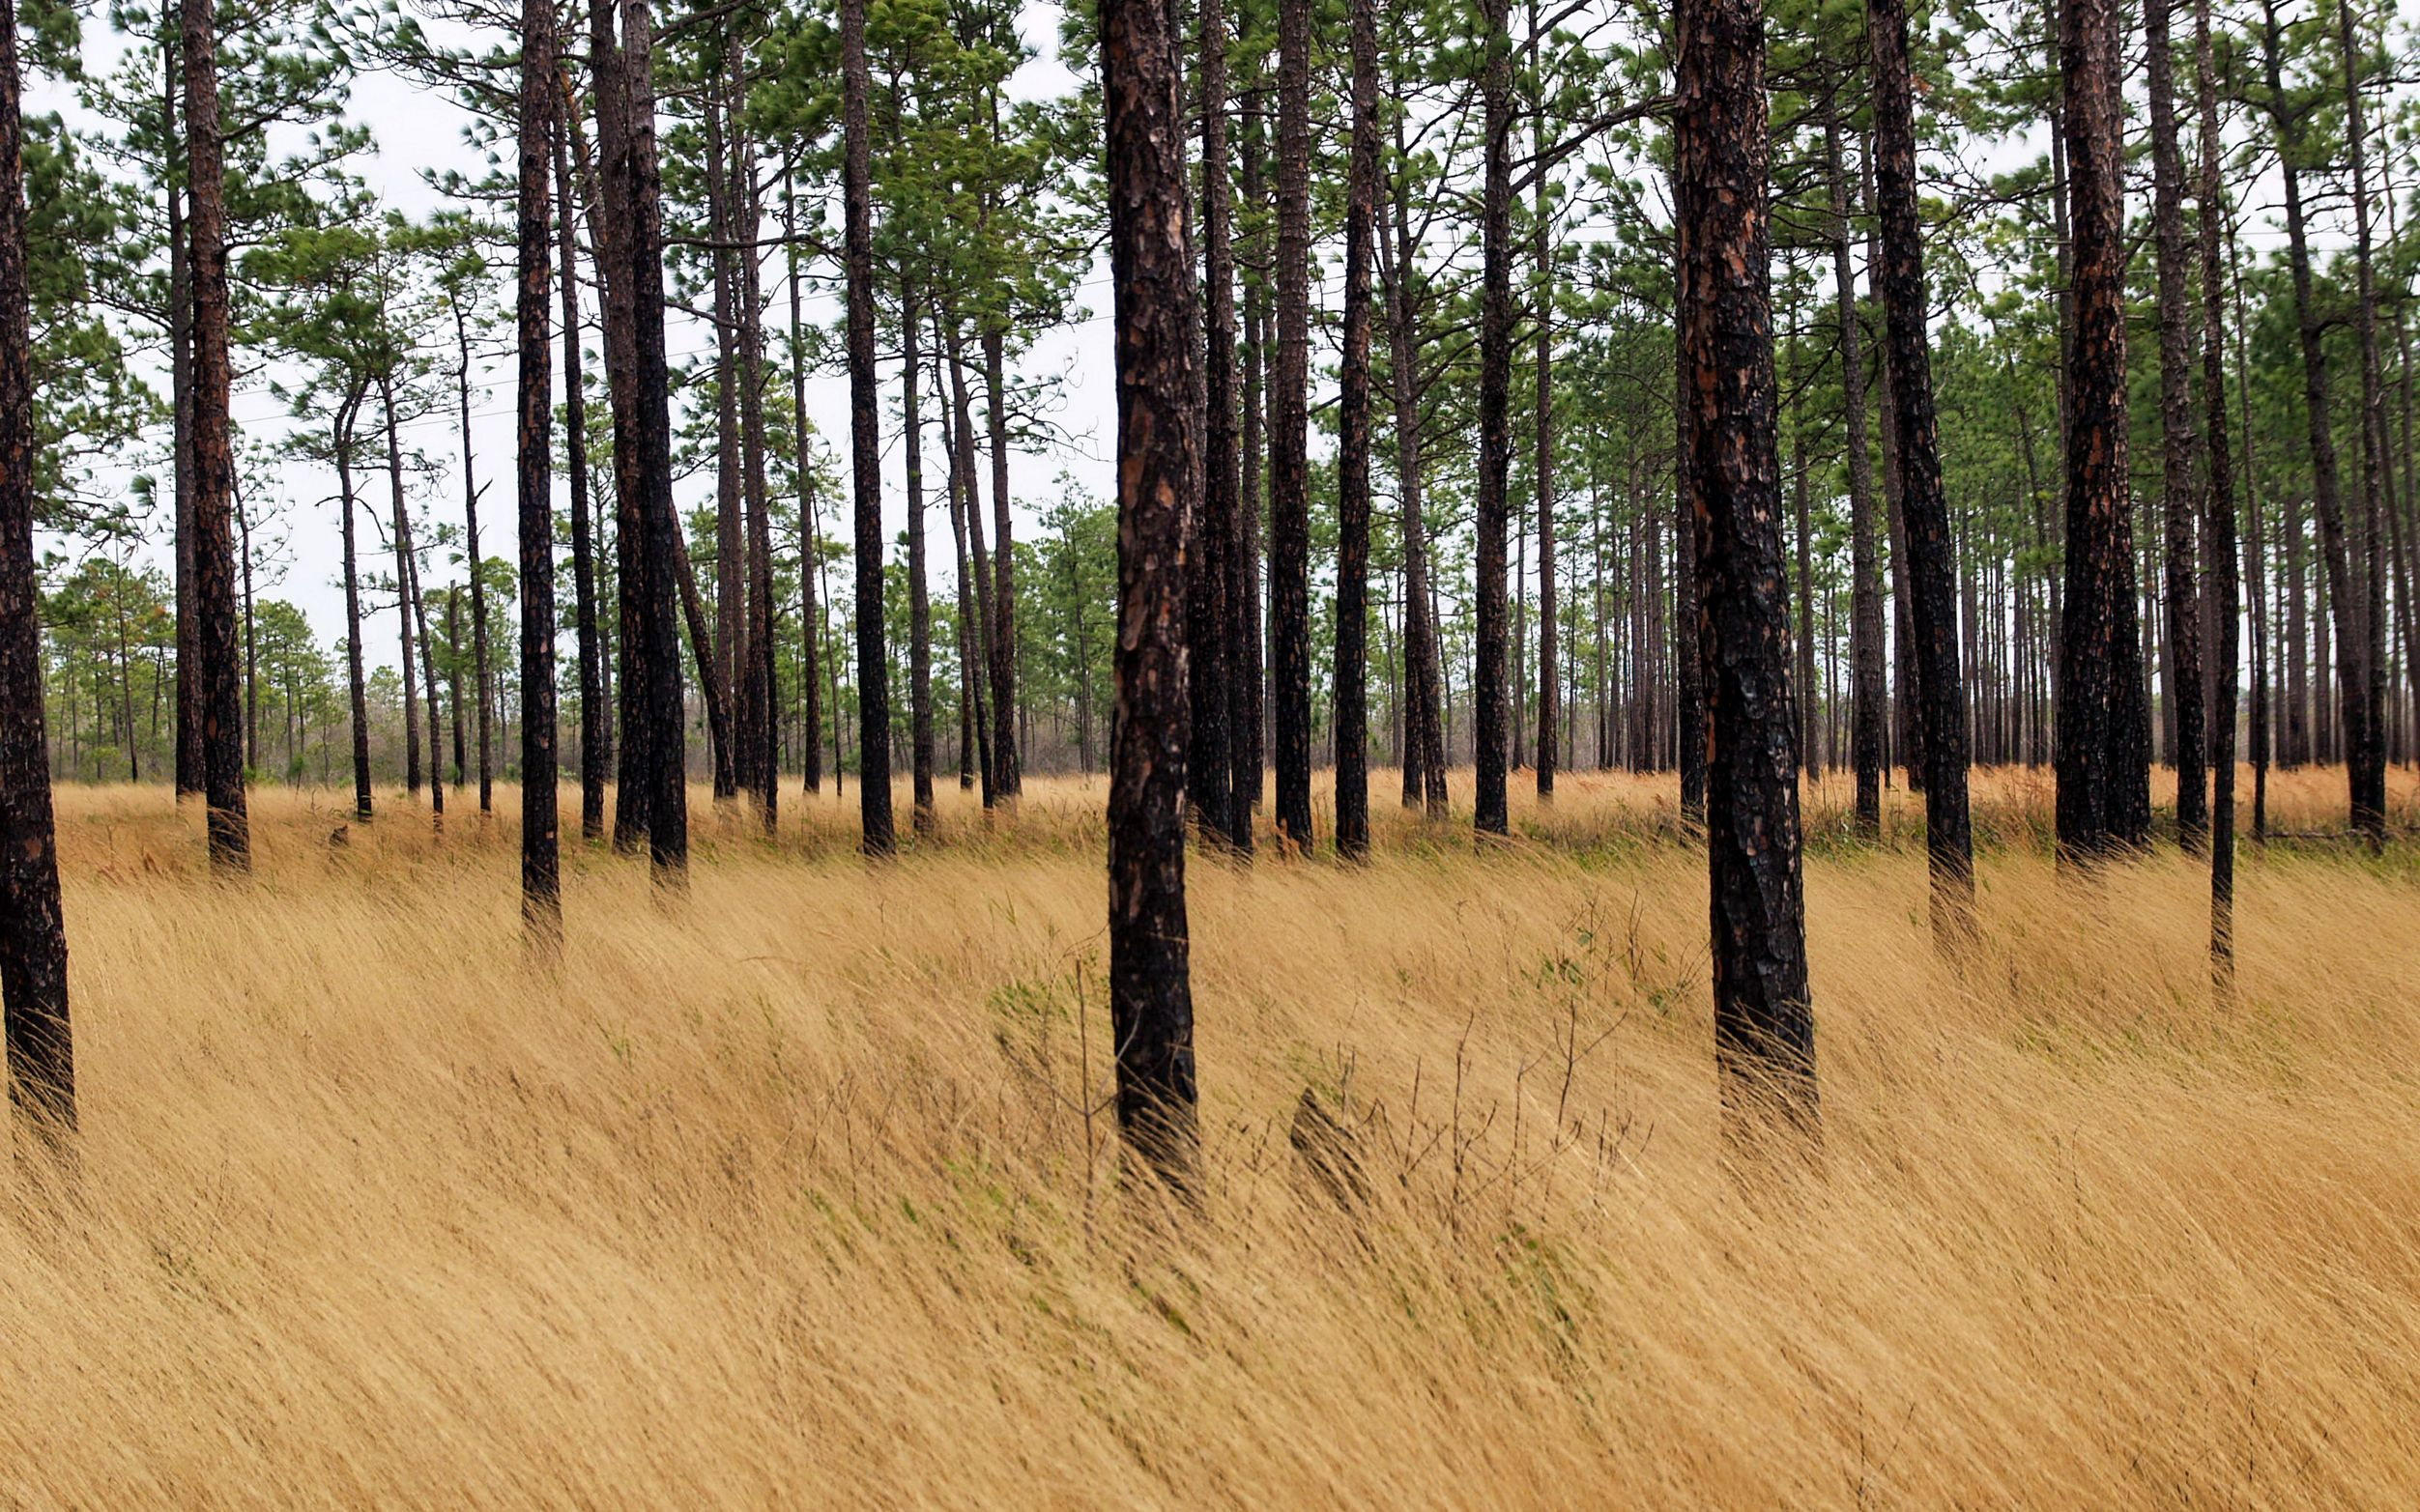
\includegraphics[width=.975\columnwidth]{SPineGrass.jpg}}
	\centerline{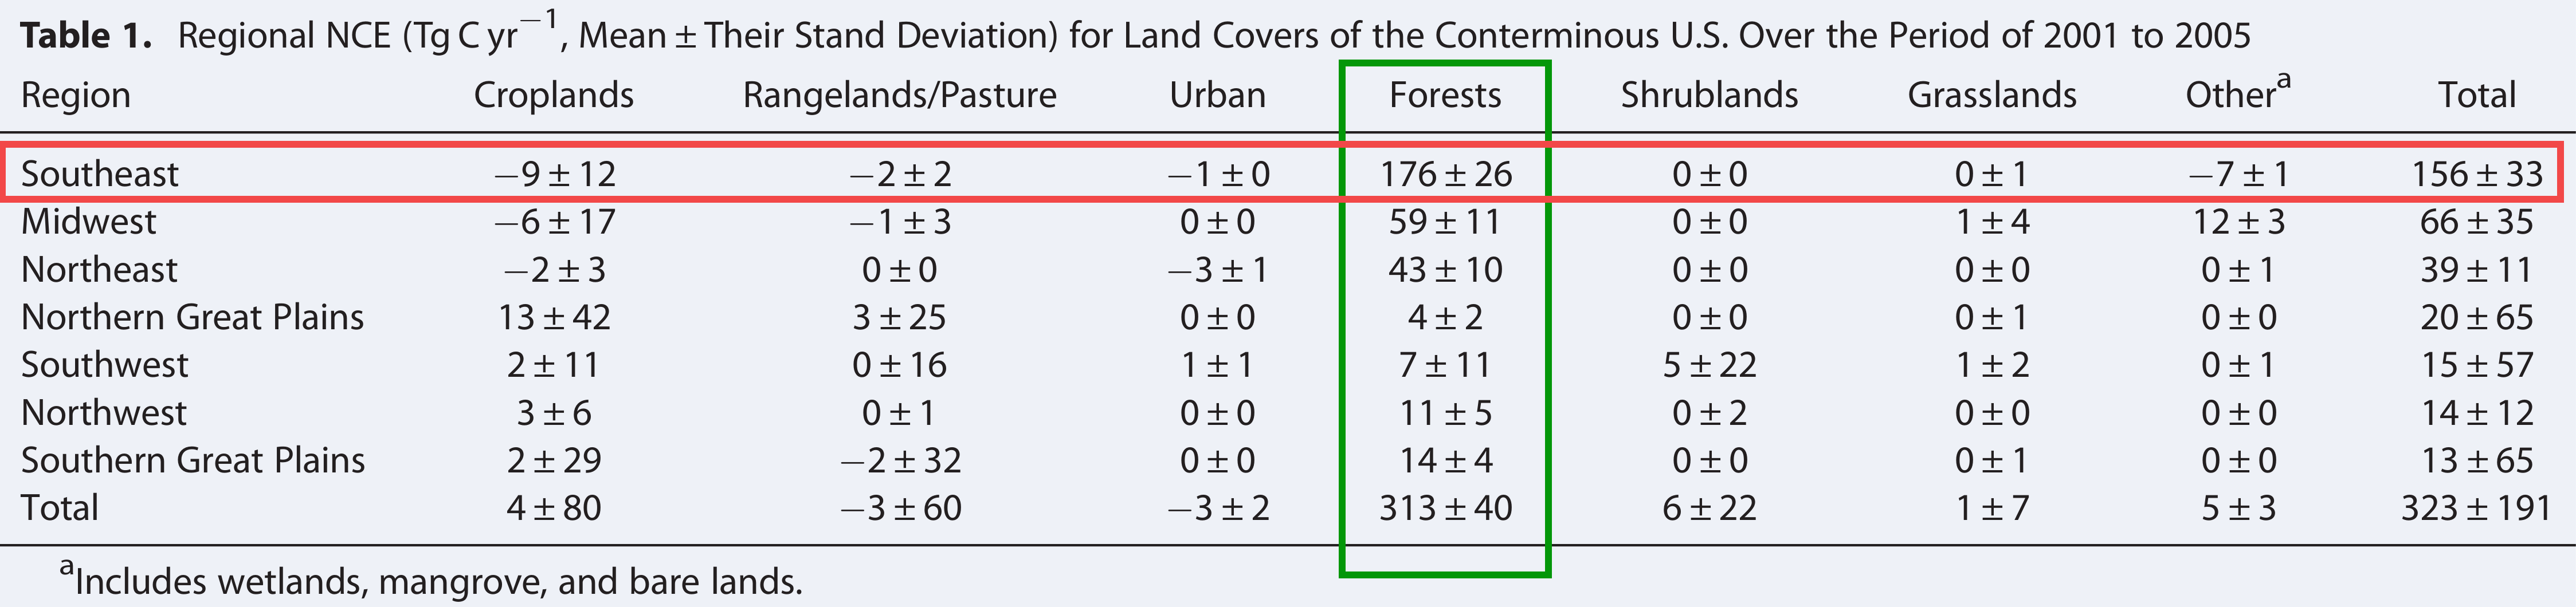
\includegraphics[width=.975\columnwidth]{CarbonForestUSRegions.png}}

	\columnbreak
		\begin{itemize}
			\item Longleaf pine (\textit{Pinus palustris}) ecosystems once occupied 90 million acres in the Southeastern United States.
			\item Timber harvest, land conversion, and wildfire suppression reduced the longleaf pine ecosystems to only 3.2 million acres. Fire is a part of their natural life cycle.
			\item Characterized by a tall overstory and a grassy forest floor, there has been a recent movement to restore these forests.
			\item Scientists have discovered that longleaf can tolerate droughts and capture more carbon than other trees, which gives them potential as a natural climate solution, especially since forests of the Southeast are already known to capture more carbon than any other forest region in the U.S.
		\end{itemize}
	\end{multicols}
\end{tcolorbox}

\begin{tcolorbox}[colback=yellow!5!white,colframe=IceCreamLeaf,title=\textbf{Hypotheses}]
	\begin{multicols}{2}
	
	\begin{itemize}
		\item Today, we are going to compare two forests. Loblolly pine is a species used by the forest products industry and longleaf pine is a species researchers hope to restore to mitigate climate change. We are going to compare longleaf pine in a wet coastal site to loblolly pine in a dry upland site.
		\item Given what you have just read, write predictions about: 
            \item[1)] How would you predict the water use efficiency to compare between the two species? Why might you expect this? 
            \item[2)] How would you predict the transpiration, evaporation, and interception (i.e., the components of ET) to compare between the two sites? Why might you expect this? 
	\end{itemize}

 
	\columnbreak

	\centerline{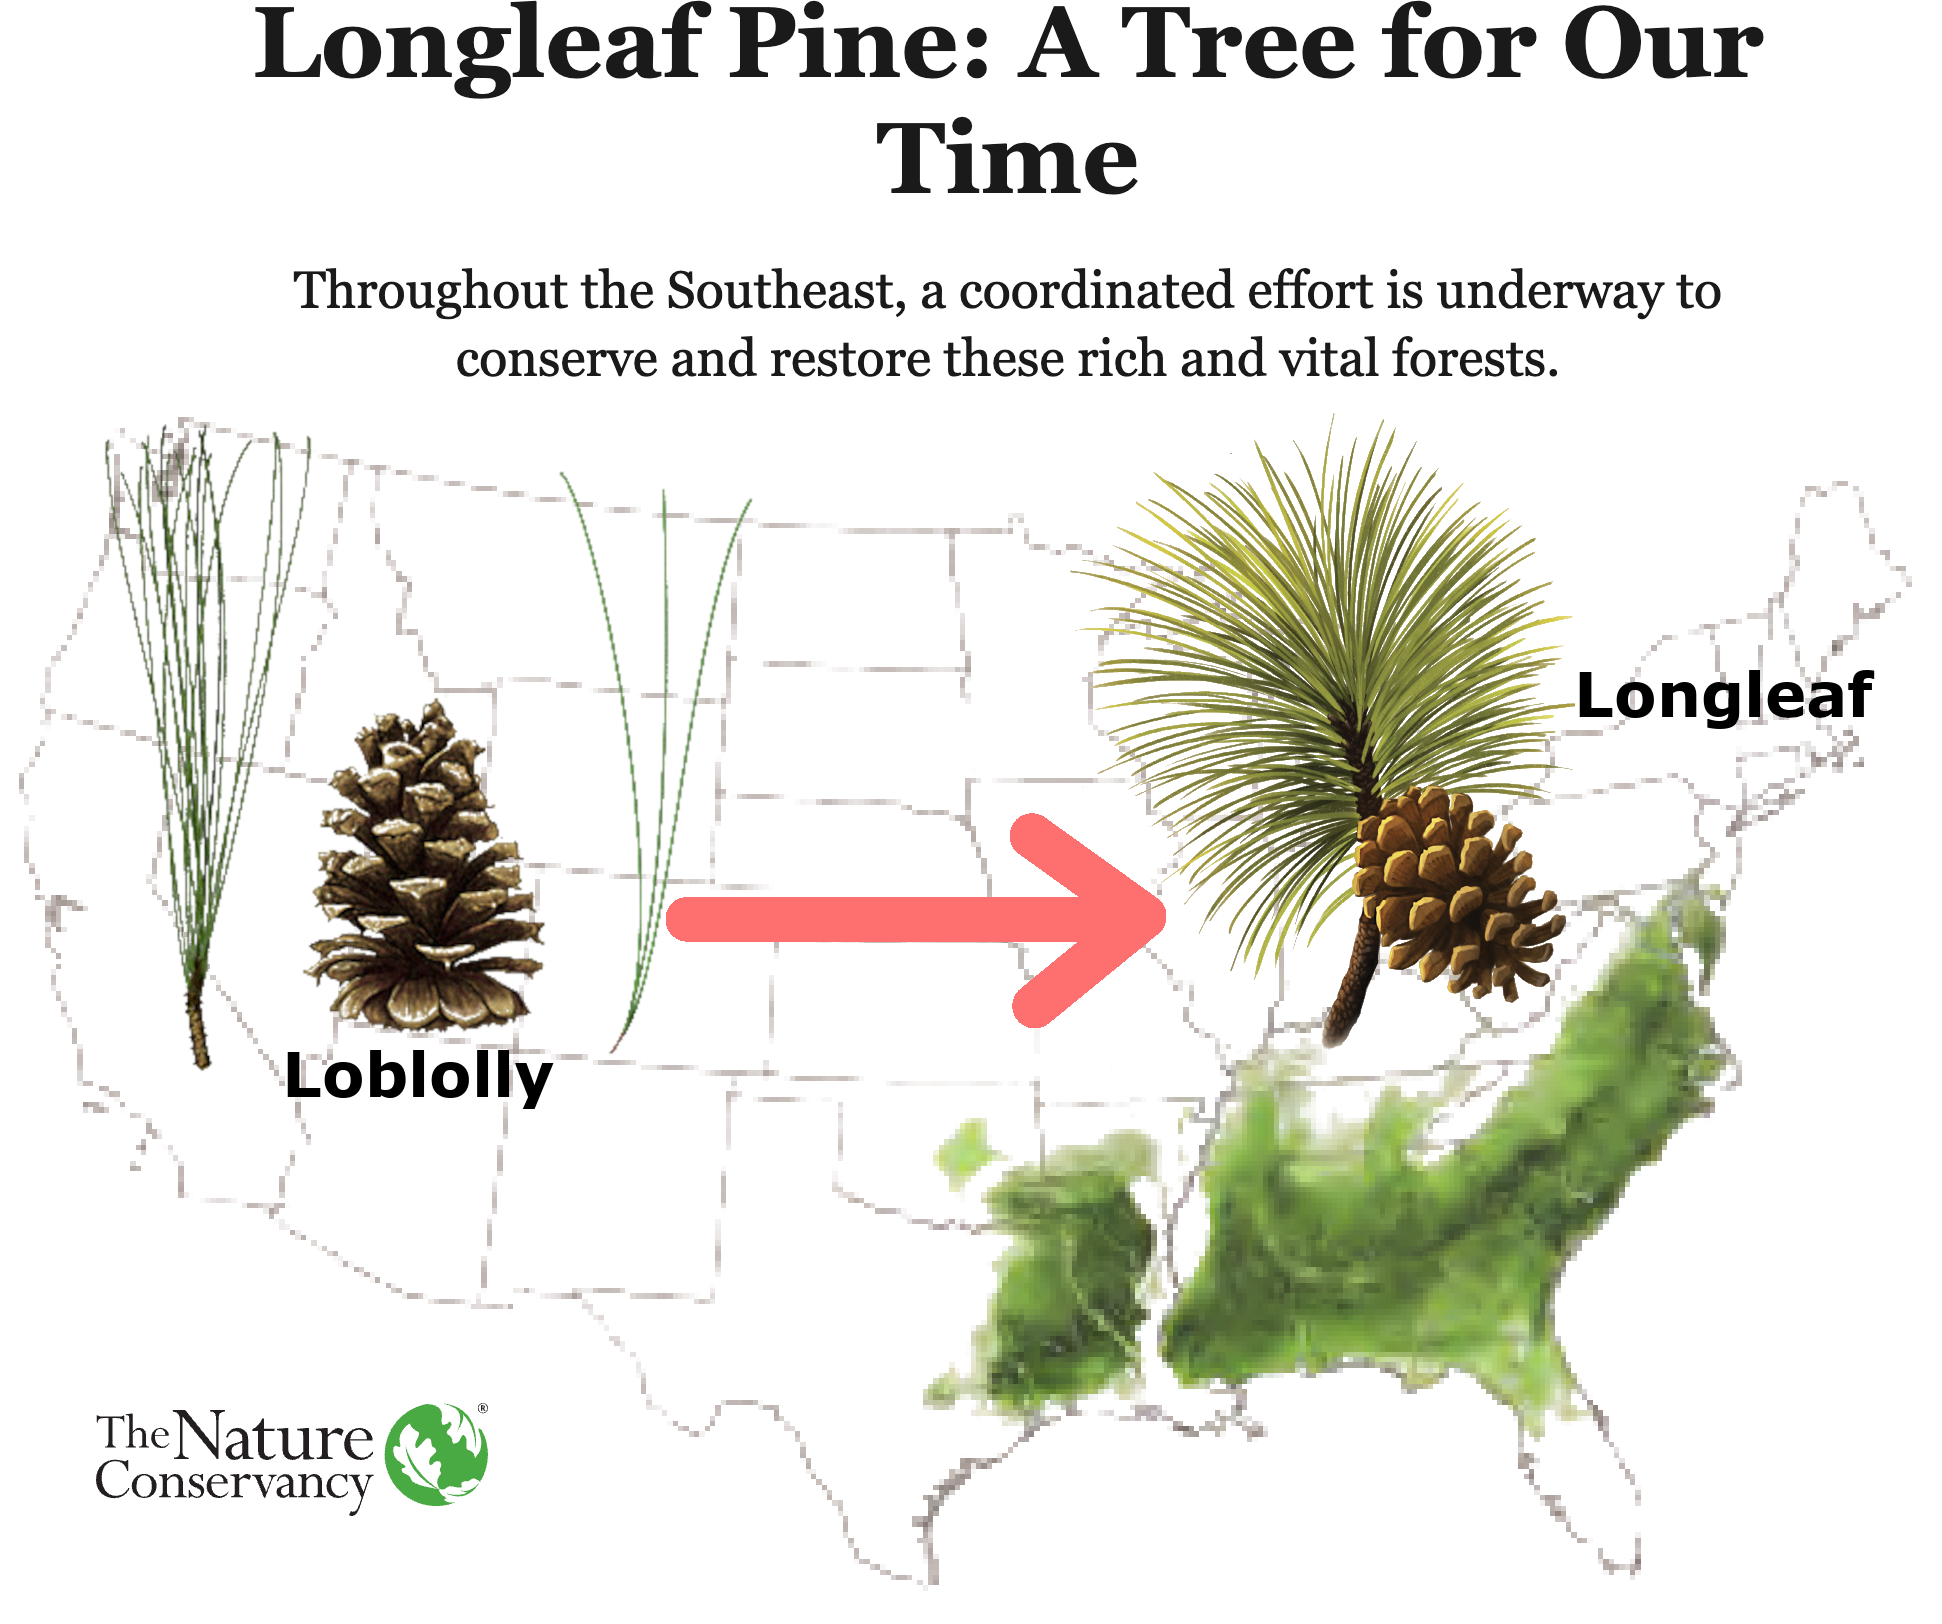
\includegraphics[width=\columnwidth]{SouthernPineIntro.png}}

	\begin{itemize}
              \item You should write down your predictions and submit them as part of your ``Map of the Week'' assignment.
	\end{itemize}

	\end{multicols}
\end{tcolorbox}


\subsection{Requesting loblolly pine ET \& WUE data from A$\rho\rho$EEARS}

The procedure for downloading ET component and WUE data through the A$\rho\rho$EEARS interface is the same as in the previous tutorials on land surface temperature.

1. First, begin by downloading these two GeoJSON files, saving them somewhere you can remember (as always, we suggest creating a folder for each tutorial):

\begin{enumerate}
	\item Longleaf Pine (South Carolina Wet Coastal Environment): \href{https://jeremydforsythe.github.io/icecream-tutorials/Tutorial10_Evapotranspiration2/LongleafSC Shapefile/LongleafSC.geojson}{LongleafSC.geojson}
	\item Loblolly Pine (North Carolina Dry Upland Environment): \href{https://jeremydforsythe.github.io/icecream-tutorials/Tutorial10_Evapotranspiration2/LoblollyNC Shapefile/LoblollyNC.geojson}{LoblollyNC.geojson}
\end{enumerate}
 

\kulbox{\textbf{NOTE:} Depending on your web browser, you may need to right click and select \textit{Save as}. Some web browsers may even display the contents of the GeoJSON file instead of prompting you to save it. If this happens, you can select the \textit{File} dropdown menu and click on \textit{Save as}. }

2. Go to \href{https://appeears.earthdatacloud.nasa.gov/}{https://appeears.earthdatacloud.nasa.gov/} and login with your credentials. 

\centerline{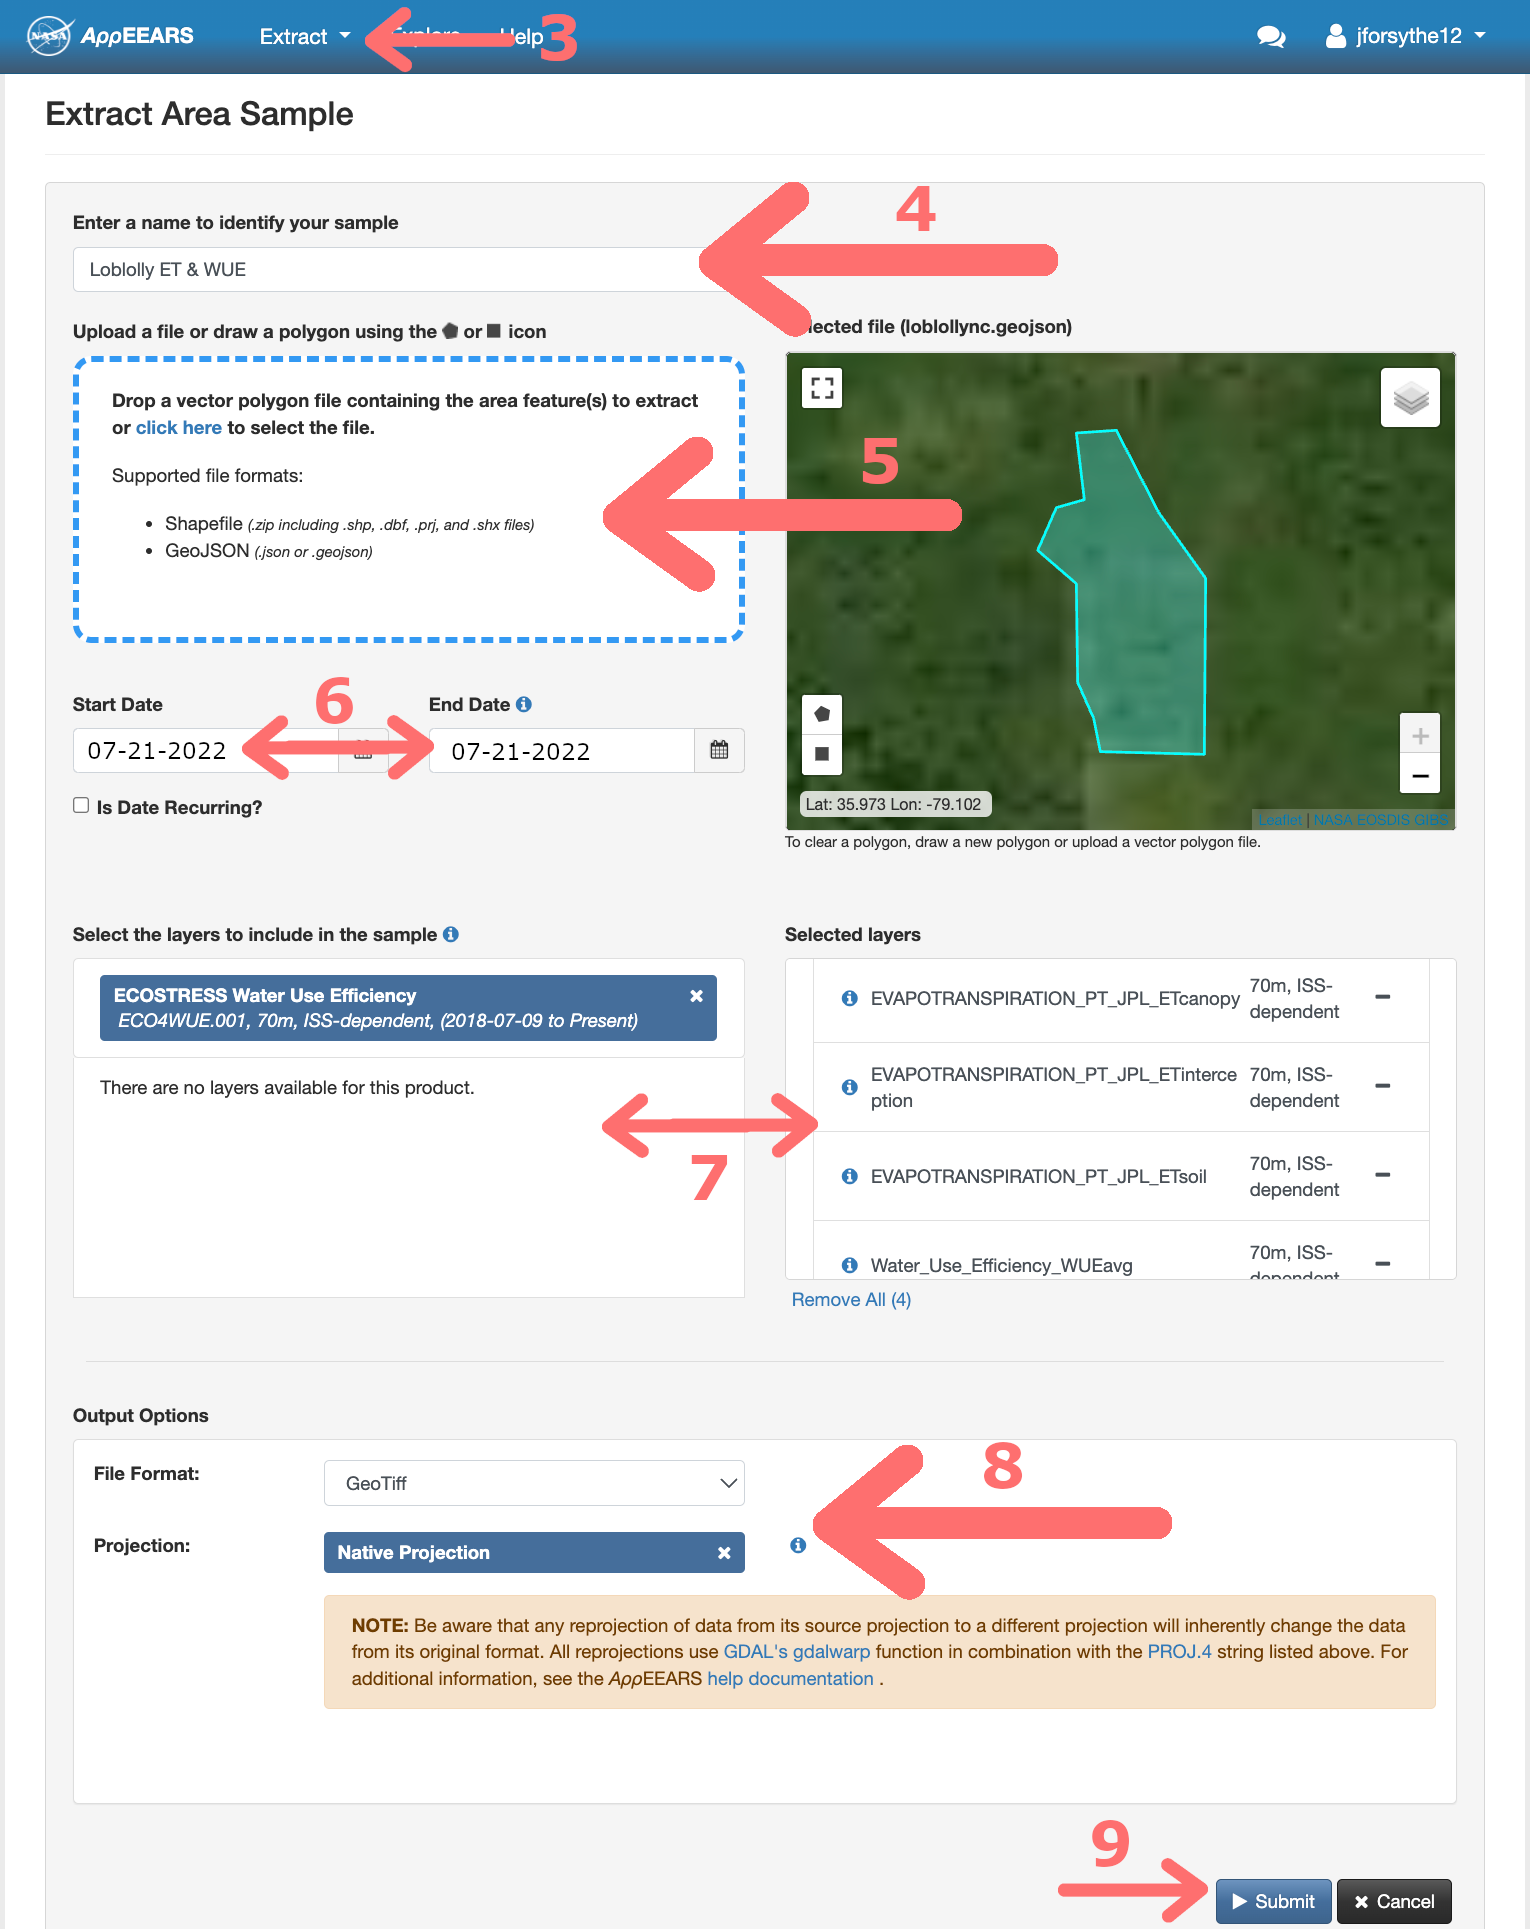
\includegraphics[width=.6\textwidth]{WUERequest.png}}

3. Use the \textit{Extract} dropdown menu to select \textit{Area}. Next, select \textit{ Start a new request}. 

4. Enter a useful name for the request you are going to submit, maybe something like ``Loblolly ET and WUE''. 

5. Drag and drop (or use the \textit{click here to select the file} link) to upload the GeoJSON file \textit{LoblollyNC.geojson}. The map should be updated with a polygon around a forest in North Carolina.

6. Update the \textit{Start} and \textit{End} Date Fields for our preselected date of interest: 07/21/2022 to 07/21/2022.

7. Under \textit{Select the layers to include in the sample} type the words ``ECOSTRESS'' and ``Evapotranspiration.'' Select \textit{ECOSTRESS Evapotranspiration PT-JPL}. Click on the ``+'' signs to add the following layers to your cart: 

\begin{itemize}
	\item $EVAPORTRANSPIRATION\_PT\_JPL\_ETcanopy$
	\item $EVAPORTRANSPIRATION\_PT\_JPL\_ETinterception$
	\item $EVAPORTRANSPIRATION\_PT\_JPL\_ETsoil$
\end{itemize}

Next, clear the selection of the current category using the small ``x'' to the right of the \textit{ECOSTRESS Evapotranspiration PT-JPL} box.

Then, under \textit{Select the layers to include in the sample} type the words ``ECOSTRESS'' and ``WUE.'' Select \textit{ECOSTRESS Water Use Efficiency}. Click on the ``+'' signs to add the following layers to your cart: 

\begin{itemize}
	\item $Water\_Use\_Efficiency\_WUEavg$
\end{itemize}

Clear the selection of the current category using the small ``x'' to the right of the \textit{ECOSTRESS Water Use Efficiency} box.

8. Under \textit{Output Options}, we want to use GeoTIFF (Geographic Tagged Image File Format; essentially an image file where the corresponding geographic information is embedded in the file) and \textit{Native Projection} for projection.

9. Click \textit{Submit} to complete the data request. At the top, you should see a green banner:

\vspace{.5em}

\centerline{
\includegraphics[width=\textwidth]{RequestSuccess.png}}

\subsection{Requesting longleaf ET \& WUE data from A$\rho\rho$EEARS}

10. In the meantime, we are going to create a second request for this tutorial, as we need data for longleaf pines to compare to the loblolly pine data we just requested. Use the \textit{Extract} dropdown menu to select \textit{Area}. Next select \textit{Start a New Request}.  Enter a useful name to distinguish this request from the other, maybe something like ``Longleaf ET and WUE''. Drag and drop (or use the \textit{click here to select the file} link) to upload the GeoJSON file \textit{LongleafSC.geojson}. The map should be updated with a polygon around a forest on the coast of South Carolina.

11. Repeat steps 6 - 9 above to retrieve the ET component and WUE data for the longleaf pine site on 7/26/2022.


\kulbox{\textbf{NOTE:} You may have noticed the dates are different for the longleaf and loblolly sites. Unfortunately, the two sites are too far apart to have a pass on the same day.}


12. Use the \textit{Explore} drop-down at the top to monitor the status of your request. Requests will likely go quickly, given that it is only one day's worth of data.

\vspace{.5em}

\centerline{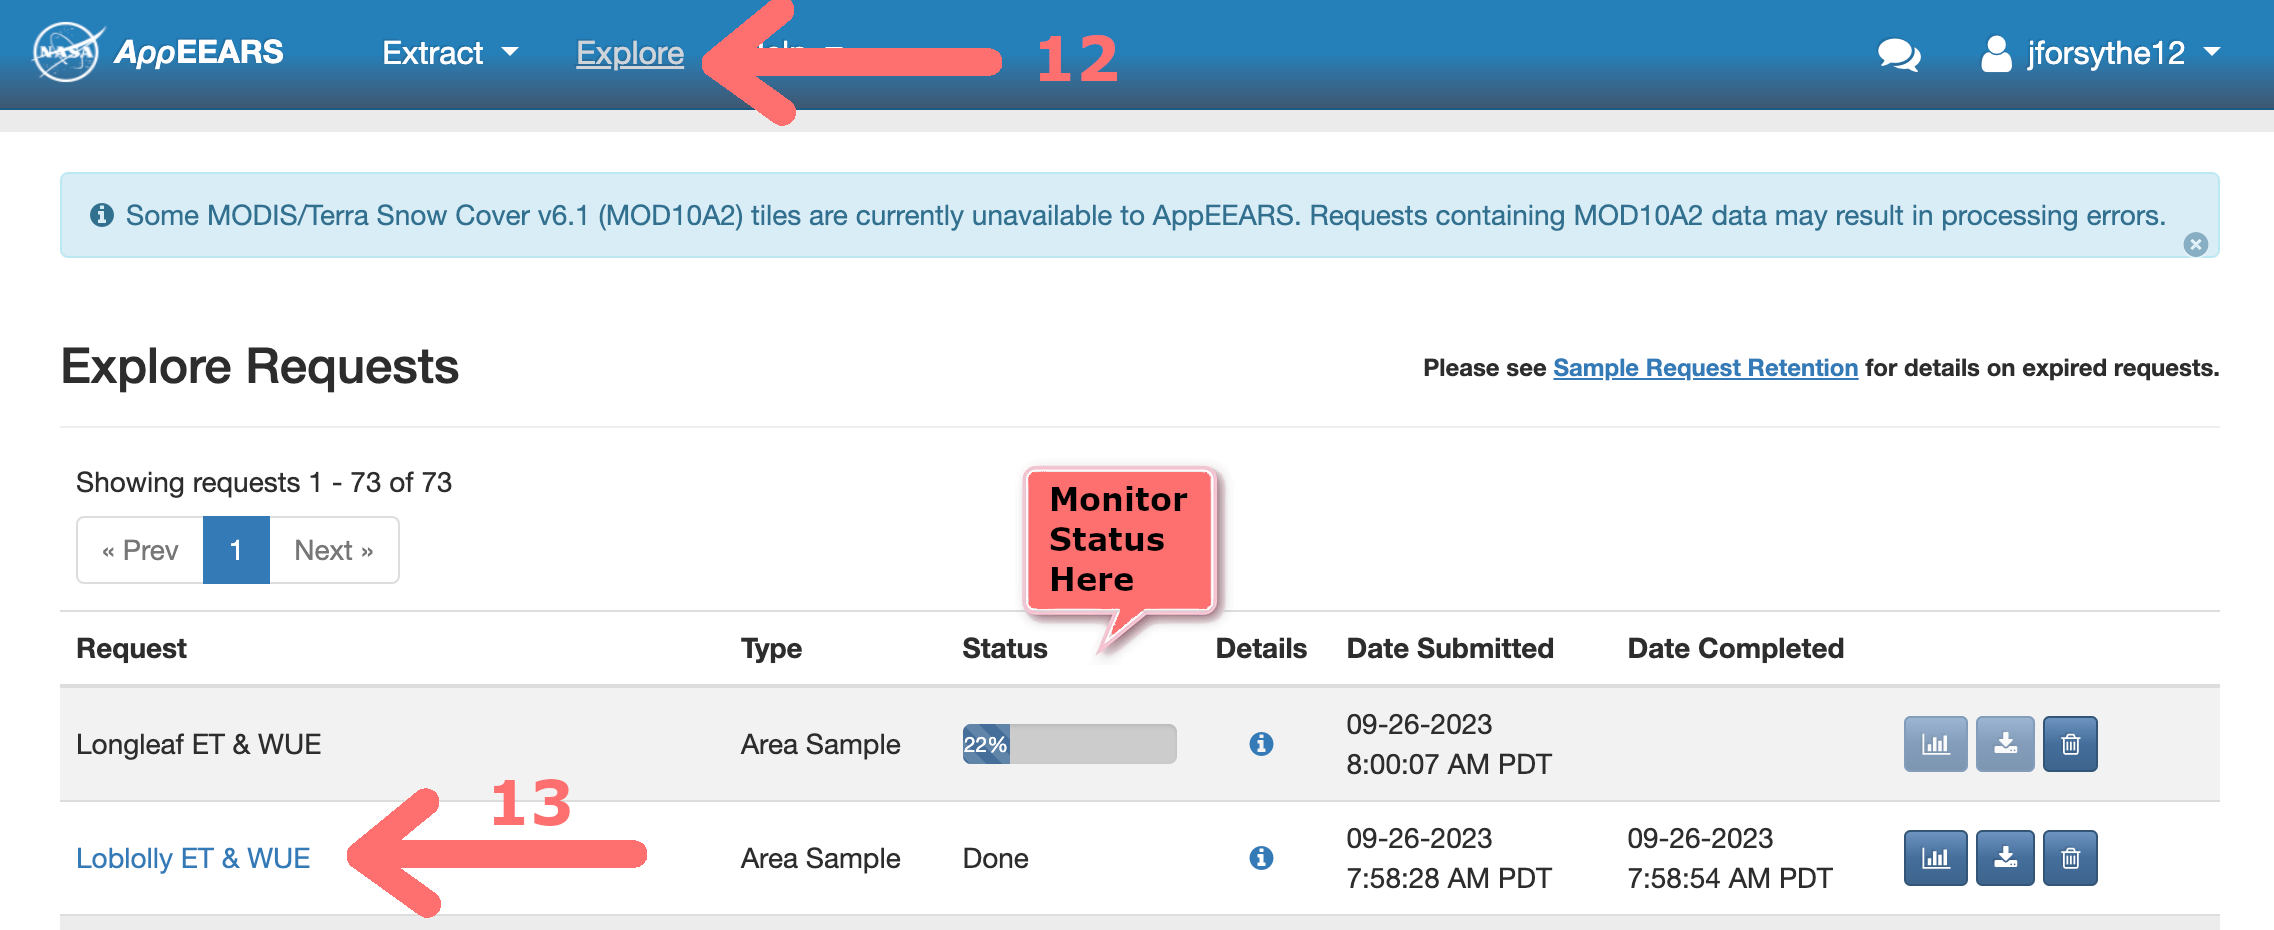
\includegraphics[width=.55\textwidth]{ExploreComplete.png}}

\vspace{.5em}

\subsection{Visualizing loblolly pine ET Component Data in A$\rho\rho$EEARS}

13. When your first request (``Loblolly ET and WUE'') is complete, use the link on the \textit{Explore} page to access the details. Let's check out the data. First, a quick review of boxplots:

\vspace{1em}

\centerline{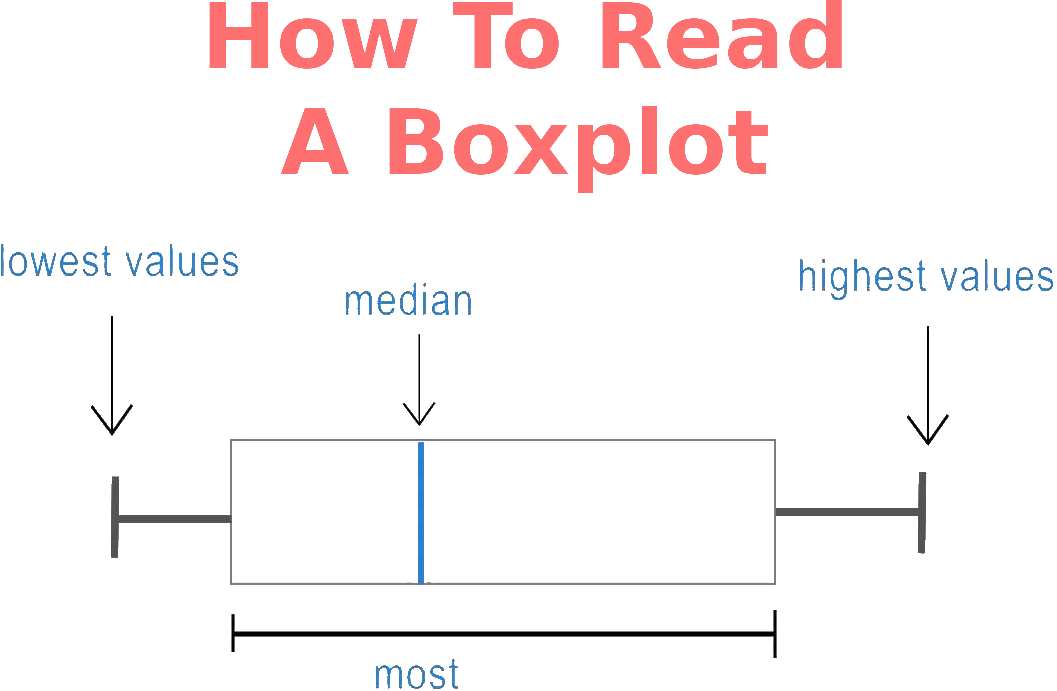
\includegraphics[width=.45\textwidth]{HowToBoxplot.png}}

\vspace{.5em}

14. Our goal for the analysis of the evapotranspiration components is not to visualize the data in space, but rather to compare the differences between the two forest ecosystems (loblolly vs. longleaf pine) as a whole. As a result, there is no need to download the GeoTIFF files and import the layers into QGIS. We can explore the data with the A$\rho\rho$EEARS interface to get the information we need.

15. First, select the $EVAPOTRANSPIRATION\_PT\_JPL\_ETcanopy$ layer:

\vspace{.5em}

\centerline{\includegraphics[width=.6\textwidth]{ETComponents.png}}

\vspace{.5em}

Notice that the median value for the canopy component of evapotranspiration is 49.57. This means that the median value for pixels in our area of interest is 49.57, which means that 49.57\% of the total evapotranspiration (the ``EVAPOTRANSPIRATION\_PT\_JPL\_ETinst'' variable) is coming from canopy transpiration. Although the overall distribution of the data is skewed towards higher values, there is no need to worry, as the range of the data (minimum to maximum observed value) is about 3\%. Since our analysis is mostly concerned with the relative percentages of the different components of ET (canopy vs. interception vs. soil), it is reasonable to simply use the median value.

16. Next, select the $EVAPOTRANSPIRATION\_PT\_JPL\_ETinterception$ layer. 

\vspace{.5em}

\centerline{\includegraphics[width=.6\textwidth]{ETComponents2.png}}

\vspace{.5em}

Here, we observe that 41.24\% of total evapotranspiration is coming from interception.

17. Finally, select the $EVAPOTRANSPIRATION\_PT\_JPL\_ETsoil$ layer.

\vspace{.5em}

\centerline{\includegraphics[width=.6\textwidth]{ETComponents3.png}}

\vspace{.5em}

So, the overall breakdown for the individual components of evapotranspiration is 49. 57\% canopy transpiration, 41. 24\% interception evaporation, and 9. 15\% soil evaporation. You will report this in the write-up that accompanies your ``Map of the Week'' assignment along with longleaf pine data that you will complete on your own. 

\subsection{Downloading loblolly pine WUE Data}

18. From the \textit{Layer} dropdown menu, choose ``Water\_Use\_Efficiency\_WUEavg'', then expand the \textit{Request} box above by clicking on the caret. Click the download button to continue.

\vspace{.5em}

\centerline{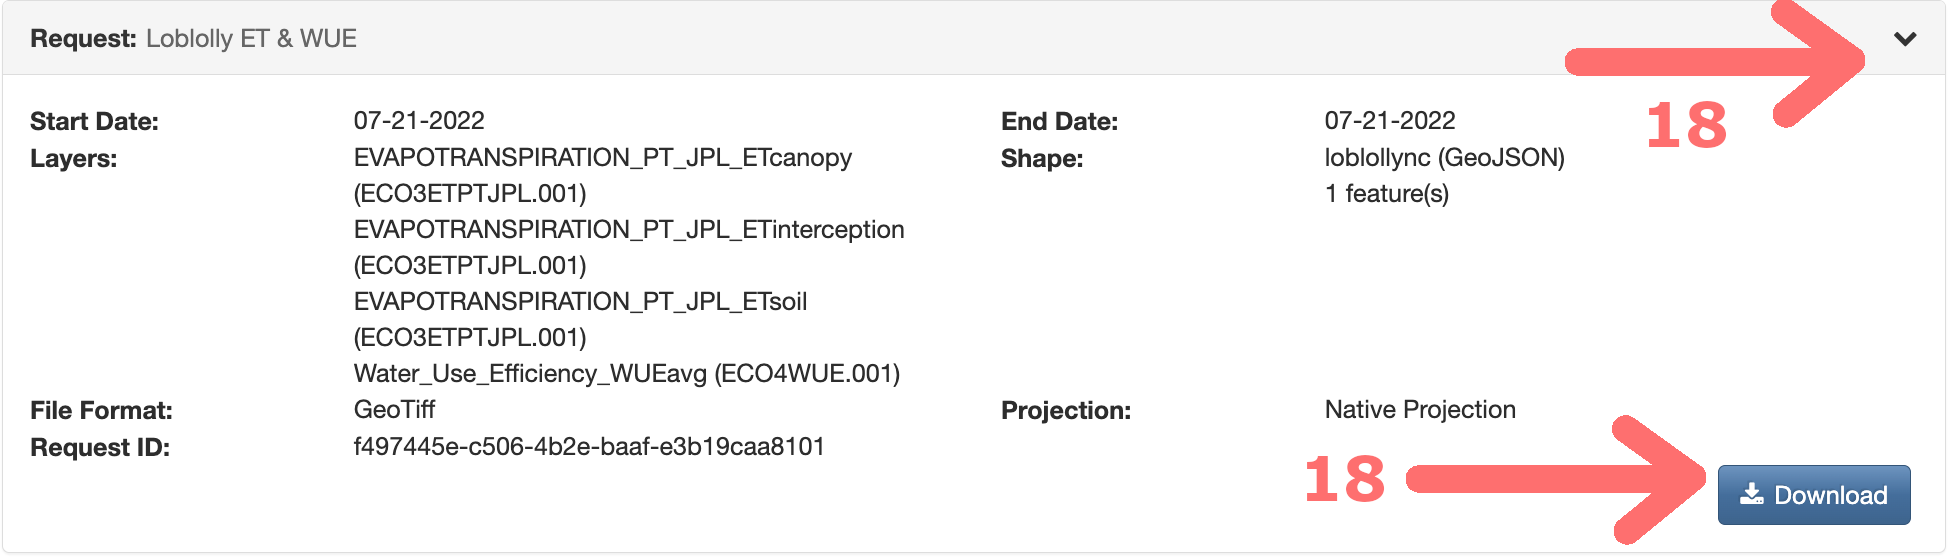
\includegraphics[width=.6\textwidth]{RequestDownload.png}}

\vspace{.5em}

\vspace{.5em}

\centerline{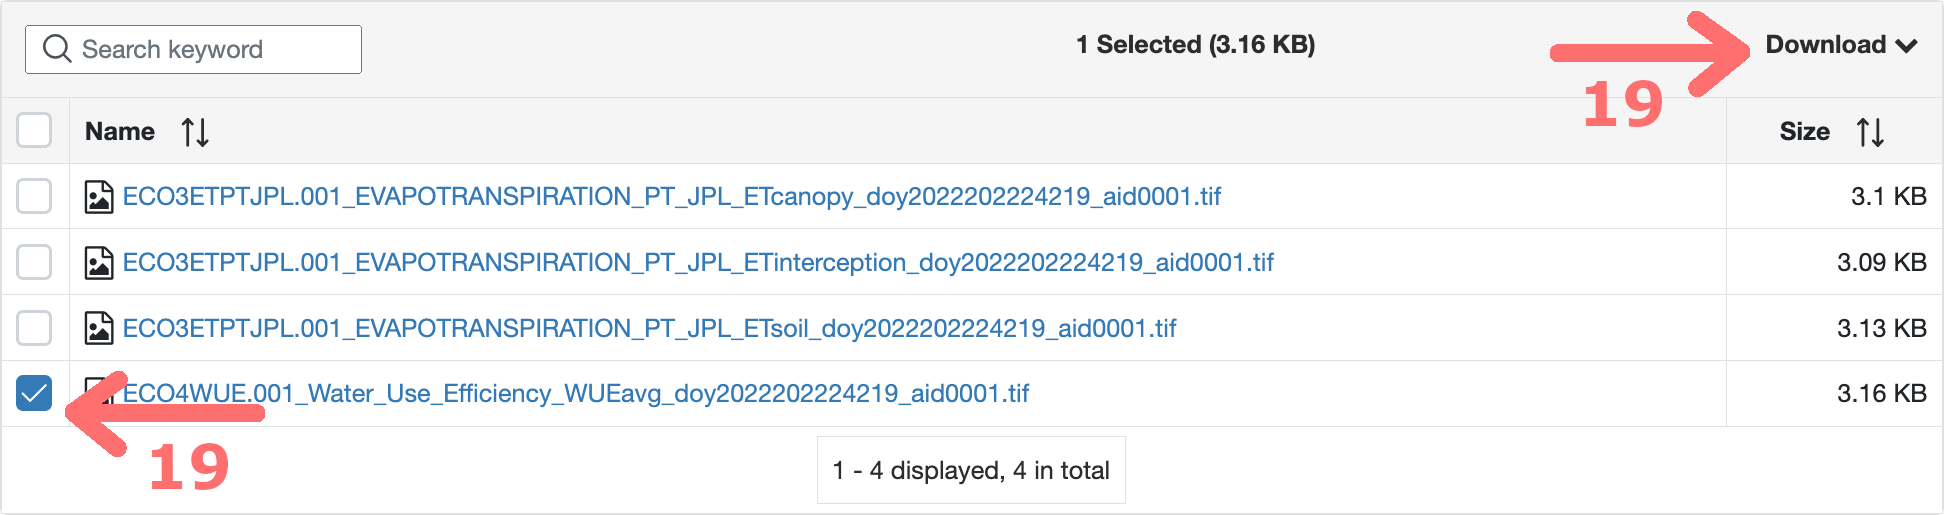
\includegraphics[width=.6\textwidth]{WUEDownload.png}}

\vspace{.5em}

19. Select the following filename: ECO4WUE.001\_Water\_Use\_Efficiency\_WUEavg\_doy2022202224219\_aid0001.tif. Download the files using the \textit{Download} button, that for some reason does not look much like a button, on the top right corner of the screen. Save the files somewhere you can remember. 

\section{Visualizing ECOSTRESS WUE Data in QGIS}

\subsection{Adding a Google Satellite Basemap}

20. Open QGIS and start a new project by selecting the \textit{Project} menu, then \textit{New}.

21. To add a basemap, find the \textit{HCMGIS} menu bar, select \textit{Basemap}, then pick your preferred map. For today's map, we will use \textit{Google Satellite}. Note that clicking on a basemap type automatically adds a new layer to your map, as seen in the layer browser window.

\vspace{.5em}

\centerline{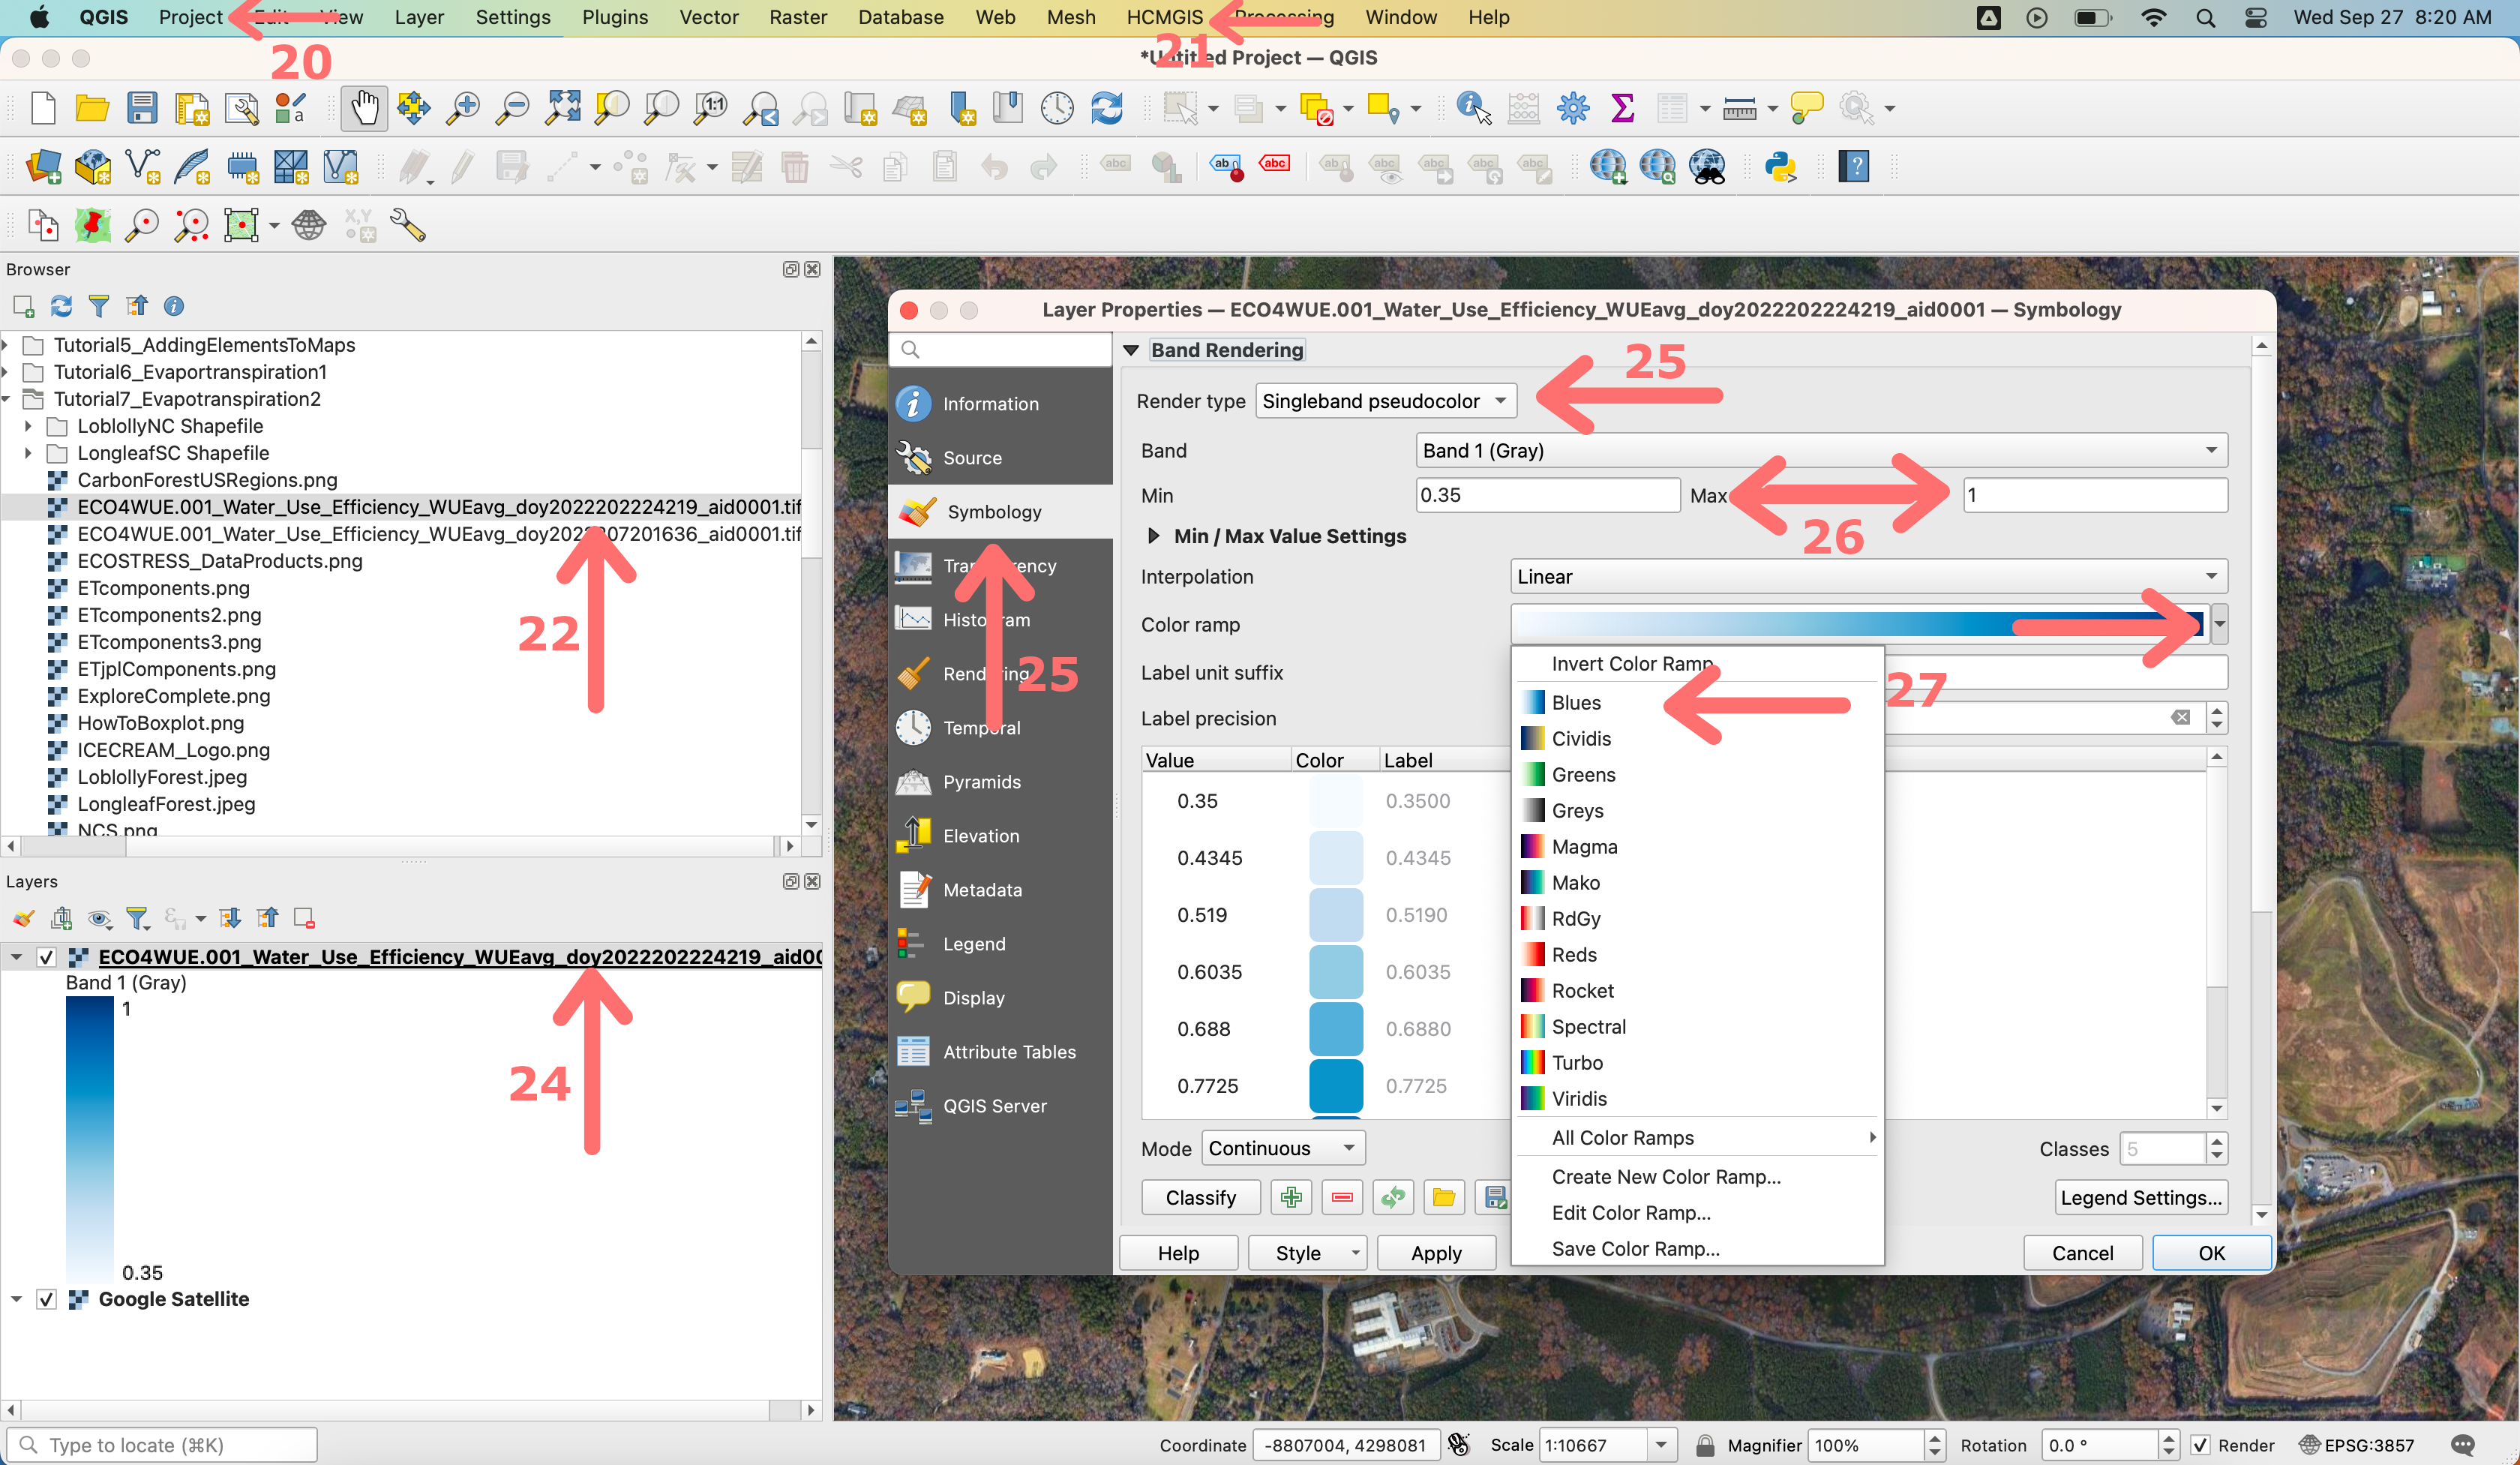
\includegraphics[width=\textwidth]{WUELayer.png}}

\subsection{Add in WUE layer}

22. Use the \textit{browser} window to find the folder where you saved the WUE file: \\ ECO4WUE.001\_Water\_Use\_Efficiency\_WUEavg\_doy2022202224219\_aid0001.tif

23. Double-click the ECO4WUE.001\_Water\_Use\_Efficiency\_WUEavg\_doy2022202224219\_aid0001.tif file to add it to your map. Again, notice that they are now also listed in the \textit{Layers} window.

\kulbox{\textbf{NOTE:} Our loblolly data is at a pretty fine scale and might be hard to see if your basemap is zoomed out at the global scale. QGIS can automatically zoom to your layer's area of interest by right clicking (ctrl-click on Mac) on the layer and selecting \textit{Zoom to Layer(s).}}

24. Now, you have ECOSTRESS WUE data on your map, but we need to change it from grayscale. Right-click (ctrl-click on Mac) on the layer name in the \textit{Layers} window and select \textit{Layer Properties}. 

25. On the menu bar to the left, select \textit{Symbology} and change \textit{Render type} to Singleband pseudocolor. 

26. QGIS has automatically determined the minimum and maximum values from the datafiles; however, we are going to want to compare two types of ecosystems and need to match them. Specify 0.35 as the minimum and 1 as the maximum. 

27. Change the color ramp to something that you feel communicates WUE. I selected the ``Blues'' option. Click apply, then ok.

28. Finally, add the border from LoblollyNC.geojso by double clicking on it in the \textit{Browser} window. Right-click (ctrl-click on Mac) on the layer in the \textit{Layers} window and change the symbology to \textit{outline red}. 


\section{Add Map Elements}

29. Following the procedure described in \href{https://jeremydforsythe.github.io/icecream-tutorials/Tutorial5_AddingElementsToMaps/Tutorial5_AddingElementsToMaps.pdf}{Tutorial \#5 : Adding Elements To Maps}, make a professional map complete with scalebars, labels, a legend, titles, and a North arrow. Include an inset that showcases the study region (North Carolina, USA) with this WUE as a basemap. This map will be your part of your map of the week assignment.

\kulbox{\textbf{NOTE:} It is not apparent in A$\rho\rho$EEARS, but the units for WUE are $gC kg^{-1} H2O$.}

\section{Make the Same Map for Longleaf Pines}

30. Follow the same procedure (steps 13 - 29) for our other request, ``Longleaf ET \& WUE'':

\begin{enumerate}
	\item Explore data for the ET components of the longleaf pine ecosystem in the A$\rho\rho$EEARS interface to determine the relative contributions of the canopy, interception, and soil to total evapotranspiration. Note the differences between longleaf and loblolly. Submit this as part of your write-up for the ``Map of the Week''.
	\item Download the water use efficiency GeoTIFF for longleaf pines.
	\item Visualize these WUE data in QGIS.
	\item Make a second professional map with the same color ramp scale for the WUE of the longleaf pine complete with scalebars, labels, a legend, titles, and a North arrow.
	\item Submit these two maps (one for longleaf, one for loblolly) as part of your ``Map of the Week'' assignment along with the write-up described below.
\end{enumerate}

\begin{tcolorbox}[colback=yellow!5!white,colframe=IceCreamOrbit,title= \vspace{.2em} \Large Map of the Week Assignments]
	\addcontentsline{toc}{section}{Map of the Week Assignments}
	\large
	\begin{enumerate}
		\item Make a WUE map for longleaf pine of the same format as the loblolly pine map we made in the tutorial. It should include a basemap of water use efficiency with an inset that highlights the geographic region. The map should be complete with scalebars(s), north arrow(s), legend(s), title(s), and label(s). Submit this longleaf map alonside the loblolly we made in the tutorial today.
        \item Provide a 1-2 paragraph description of your maps and ET component data that includes your relections on which tree species may be better suited to mitigate climate change given any differences in water use efficiency. Would you recommend that foresters plant longleaf pine trees instead of loblolly? Will longleaf pines have higher growth while minimizing water use? Address the limitations of your analysis.
	\end{enumerate}
\end{tcolorbox}

\begin{tcolorbox}[colback=yellow!5!white,title=\textbf{Datafiles}]
	\addcontentsline{toc}{section}{Datafiles}
	\large
	In case you encountered any issues with the A$\rho\rho$EEARS database, here are copies of the ECOSTRESS GeoTIFF file for the loblolly WUE:
	\begin{enumerate}
		\item \href{https://jeremydforsythe.github.io/icecream-tutorials/Tutorial10_Evapotranspiration2/ECO4WUE.001_Water_Use_Efficiency_WUEavg_doy2022202224219_aid0001.tif}{\small ECO4WUE.001\_Water\_Use\_Efficiency\_WUEavg\_doy2022202224219\_aid0001.tif}
	\end{enumerate}
	And longleaf WUE:
	\begin{enumerate}
		\item \href{https://jeremydforsythe.github.io/icecream-tutorials/Tutorial10_Evapotranspiration2/ECO4WUE.001_Water_Use_Efficiency_WUEavg_doy2022207201636_aid0001.tif}{\small ECO4WUE.001\_Water\_Use\_Efficiency\_WUEavg\_doy2022207201636\_aid0001.tif}
	\end{enumerate}
\end{tcolorbox}

%%%%%%%%%%%%%%%%%%%%%%%%%%%%%%%%%%%%%%%%%%%%%%%%%%%%%%%%%%%%%%%%%%%%%%%%%%%%%%%%%%% End of Document
%\vfill

\hrule

\vspace{1em}

\small \textbf{Recommended Citation:} Forsythe, J.D., G.R. Goldsmith, and J.B. Fisher. 2023. Observing Earth from Above Tutorials. Chapman University. \url{https://jeremydforsythe.github.io/icecream-tutorials/}

\vspace{1em}

This work is supported by funding from NASA ECOSTRESS Mission Grant \#80NSSC23K0309 (I.C.E. C.R.E.A.M.: Integrating Communication of ECOSTRESS Into Community Research, Education, Applications, and Media).

\end{document}
